\pdfobjcompresslevel=1
\newcommand{\doctitle}{QGIS Instant Print Plugin}
\newcommand{\docauthor}{Sandro Mani}

\documentclass[11pt,twoside,a4paper]{report}
%Language, input
\usepackage[english]{babel}
\usepackage[utf8]{inputenc}
\usepackage[T1]{fontenc}
\selectlanguage{english}
%\mathcode`\.="613A	% Uncomment if using coma as decimal separator
%\mathcode`\,="013B	% Uncomment if using dot as decimal separator

%Geometry, Documentstyle
\usepackage{geometry,rotating,tabls}
\geometry{a4paper,twoside=true,inner=3cm,outer=2cm}
\setlength{\headheight}{14pt}
\addtolength{\voffset}{-1cm}
\addtolength{\textheight}{4cm}
\linespread{1.3} \sloppy
\parindent=0cm
\setlength{\parskip}{1.5ex}


%Headers, Footers
\usepackage{fancyhdr}
\pagestyle{fancy} \fancyhf{}
\fancyhead[L]{\doctitle}
\fancyhead[R]{
\includegraphics[width=.25\textwidth]{logo_text.pdf}}
\renewcommand{\footrulewidth}{0.4pt}
\fancyfoot[R]{\nouppercase{\thepage}}

\fancypagestyle{plain}{
\pagestyle{fancy} \fancyhf{}
\fancyhead[L]{\doctitle}
\fancyhead[R]{
\includegraphics[width=.25\textwidth]{logo_text.pdf}}
\renewcommand{\footrulewidth}{0.4pt}
\fancyfoot[R]{\nouppercase{\thepage}}
}


%Graphics, Pictures
\usepackage{color,graphicx}
\usepackage[footnotesize,hang,it]{caption}
\setlength{\captionmargin}{20pt}
\graphicspath{{img/}}

%Footnotes, Lists
\usepackage{footnote,paralist,enumerate}
\usepackage[stable]{footmisc}
\makesavenoteenv{tabular}
\makesavenoteenv{figure}
\makesavenoteenv{itemize}

%Index, Bibliography
\usepackage{makeidx,tocbibind} % Use \tableofcontents resp \makeindex
\makeindex

%Hyperref
\usepackage[pdftitle={\doctitle},pdfauthor={\docauthor, Sourcepole AG},pdfdisplaydoctitle={false}]{hyperref}
\hypersetup{colorlinks=false,linkcolor=blue,anchorcolor=red,citecolor=blue,filecolor=red,urlcolor=blue}

%Font
\renewcommand{\familydefault}{\sfdefault}

%Chapter style
\usepackage{titlesec,color}
\titleformat{\chapter}[hang]{\Huge\bfseries}{\thechapter\quad\textcolor[rgb]{0.75,0.75,0.75}{|}\quad}{0pt}{\Huge\bfseries}

%Misc
\usepackage{tabularx}

%%%%%%%%%%%%%%%%%%%%%%%%%%%%%%%%%%%%%%%%%%%%%%%%%%%%%%%%%%%%%%%%%%%%%%%
\begin{document}
\thispagestyle{empty}
\begin{flushright}
 
\includegraphics[width=.5\textwidth]{logo_full.pdf}\\[5mm]
 \begin{minipage}{.5\textwidth}
  \begin{center}
   \small{
   Sourcepole AG | Weberstrasse 5 | 8004 Zürich\\
   Tel. +41 44 440 77 11 | Fax +41 44 440 77 12\\
   info@sourcepole.ch | www.sourcepole.ch
   }
  \end{center}
 \end{minipage}
\end{flushright}
\vfill
{\huge{\textbf{\doctitle}}}
\vfill
\begin{tabular}{ll}
 Version: & 1.0\\
 Author: & \docauthor\\
 Date: & \today\\
\end{tabular}

\newpage

\chapter*{Usage}

The instant print plugin allows to quickly print map excerpts to a file, utilizing an existing composer as page layout.

To use the instant print tool, a composer needs to be created first. The only requirement is that it contains exactly one map item.

The instant print tool can then be activated from the plugin toolbar by clicking on the plugin icon 
\includegraphics[height=11pt]{../icons/icon.png}.

In the dialog window which appears, one can pick the composer to use as page layout. A selection rectangle is displayed in the map canvas, sized according to the size of the map item in the composer and the scale chosen in the instant print dialog. The selection rectangle can be freely dragged around to choose the region one wishes to print. When dragging the selection rectangle, the previous rectangle is shown shaded and can be used as a snap reference when setting the new region. While the instant print tool is active, the canvas can be panned with the middle mouse button.

\begin{center}
 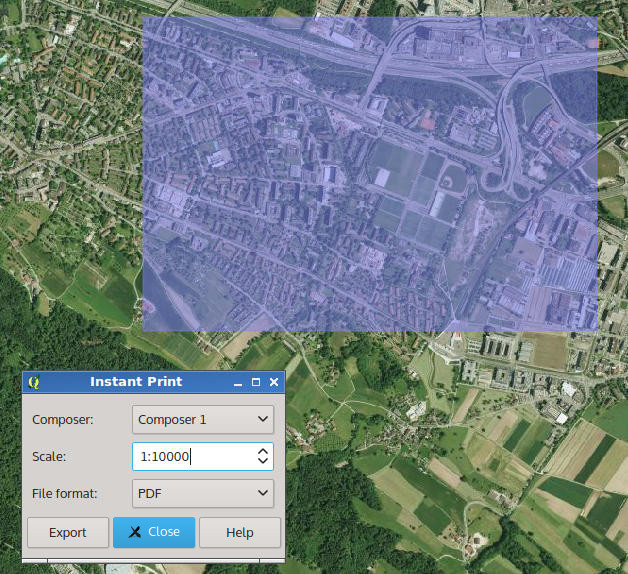
\includegraphics[width=.5\textwidth]{img/screenshot.jpg}
\end{center}


Clicking on the Export button in the instant print dialog opens a file save dialog which allows one to save the composer with the selected map excerpt.

\newpage
{\Large{\textbf{Version history}}}
{\small{
\begin{center}
\begin{tabularx}{\textwidth}{|c|c|l|X|}
 \hline
 \textbf{Version} & \textbf{Date} & \textbf{Author} & \textbf{Description} \\\hline
 1.0   & 26.02.2015 & Sandro Mani & First release \\\hline
 1.0.1 & 18.03.2015 & Sandro Mani & Ensure export filename has correct extension. \\
       &            &             & Partial workaround for QGIS bug causing crashes when closing a project with more than one composer. (To prevent crashes, make sure the Instant Print dialog is closed before closing a project.)\\\hline
 1.0.2 & 15.06.2015 & Sandro Mani & Fix cursor not unsetting after tool deactivated \\
       &            &             & Add support for PyQt4 < 4.8.4 \\\hline
 \end{tabularx}
\end{center}
}}


\end{document}
